\documentclass[12pt]{article}
% \usepackage{amsmath}
% \usepackage{hyperref}
% \usepackage[utf8]{inputenc}
% \usepackage[sfdefault]{roboto}
% \usepackage[T1]{fontenc}

% For figures
\usepackage{graphicx}
\graphicspath{{figures/}}


% For bibliography
\usepackage[numbers]{natbib}
\usepackage{url}

\usepackage{csquotes}

\title{AmDex: Reinsurance Data System}
\author{Luca Ciraolo}
\date{\today}

\begin{document}
\maketitle
\begin{abstract}
    % TODO Fix abstract
    This paper will introduce the problem which many companies face: outgrowing existing workflows. As companies scale, workflows must be modified and revised to establish more concrete solutions to ensure data integrity and cohesive functioning of employees. A specific company based in the reinsurance business facing these troubles will have their data management problems overhauled. The existing solutions will be evaluated as well as more general solutions which introduce more of the same issue: flexibility results in loss of integrity. Ultimately, a bespoke system is deemed to be necessary and an overview of the web technologies and the many moving parts that will need to be developed to create a functional, long-term, scalable solution will be presented. Finally, specific requirements of the project will be identified as well as measurable evaluation criteria which will be used to ascertain the ultimate success of the project.
\end{abstract}
\newpage

% TODO: make table of contents
% \section{Table of Contents}
\tableofcontents
\newpage

\section{Background}
This project is specific to the reinsurance industry. Knowledge of how the reinsurance industry operates is not deemed general knowledge and will therefore be explained in this section.

\begin{itemize}
    \item \blockquote[\cite{wikipedia_insurance}]{Insurance is a means of protection from financial loss. It is a form of risk management, primarily used to hedge against the risk of a contingent or uncertain loss.}
    \item \blockquote[\cite{wikipedia_reinsurance}]{Reinsurance is insurance that an insurance company purchases from another insurance company to insulate itself (at least in part) from the risk of a major claims event.}
\end{itemize}

Let us create an example scenario. A boat owner would like financial protection of their boat in case of damage so they contact an insurance company and take out an insurance policy for the vessel. The insurance policy is a contract between the boat owner and the insurance company. The owner pays the insurance company yearly (this is known as an insurance premium) so that if it is damaged, the insurance company will pay for the repairs. The insurance company has policies with 100 boat owners which allows them to amass a pool of money (reserve) from the premiums they are collecting. Then on the rare occasion that a boat is damaged, the owner will make a claim to the insurer. The insurer will then use part of the reserve to pay the claim.

The problem with this system is if there are too many claims at once. This could happen if there is a natural disaster such as a hurricane which would result in the insurer taking a large financial loss. (Note that the insurer is legally obligated to hold a minimum amount in the reserve at all times.) In order for the insurer to protect themselves against this kind of catastrophe, they will themselves take out insurance with other insurers. This is known as reinsurance. For example, the insurer might go to 4 reinsurers and take out a policy with each covering 25\% of their portfolio. This effectively spreads the risk out. Reinsurance companies can also get insurance themselves. The result of all this insurance and reinsurance is the large scale spreading of risk.


\section{Problem Introduction}
AM RE Syndicate Inc.\cite{amre} is a Managing General Agent (MGA), a type of reinsurance company. AM RE represents a panel of International Reinsurance Companies based in Europe and Asia. These represented companies, "securities", grant AM RE the authority to seek, underwrite and manage business on their behalf under the terms of the Binding Authorities ("binders"). These "binders" specify the types of business that AM RE can reinsure as well as limits of risks or geography, maximum premium to be generated, fees, etc. Business comes to AM RE through intermediaries (reinsurance brokers).

Currently, AM RE underwrites approximately 40 contracts from 25 clients each year of account. Additionally, they must manage the run-off of previous years of account on behalf of their securities since 2014. As a consequence, they have to manage over 100 active contracts which require record keeping of results so that they can be reported to the securities quarterly. Each quarter, they record 400-500 statements of accounts and payment advice which must each be audited, evidenced by original documentation sent by intermediaries and then reconciled into their system.

AM RE has approximately 15 employees (analysts and underwriters). Currently they store all their business data in 6 large spreadsheets. This was convenient when the company was very small as the employees were all familiar with spreadsheet software but as the amount of data and size of the company grows, this workflow is becoming more and more inconvenient and inefficient. The data is spread across multiple files which requires a huge amount of human intervention to ensure data consistency. As the business is growing, increasing amounts of data need to be entered each day and because the workflow is so inefficient, AM RE has been forced to hire more people to handle the rising workload. However, this has caused another major issue with spreadsheet software to surface: only one
user can edit a file at a given time. This means that hiring more people is only a short-term solution which is not at all scalable.

\subsection{Current AM RE Workflow}
In order to define the scope and specifics of the project, we must first analyse the current workflow at AM RE and look at the issues that we aim to solve.

\begin{figure}
    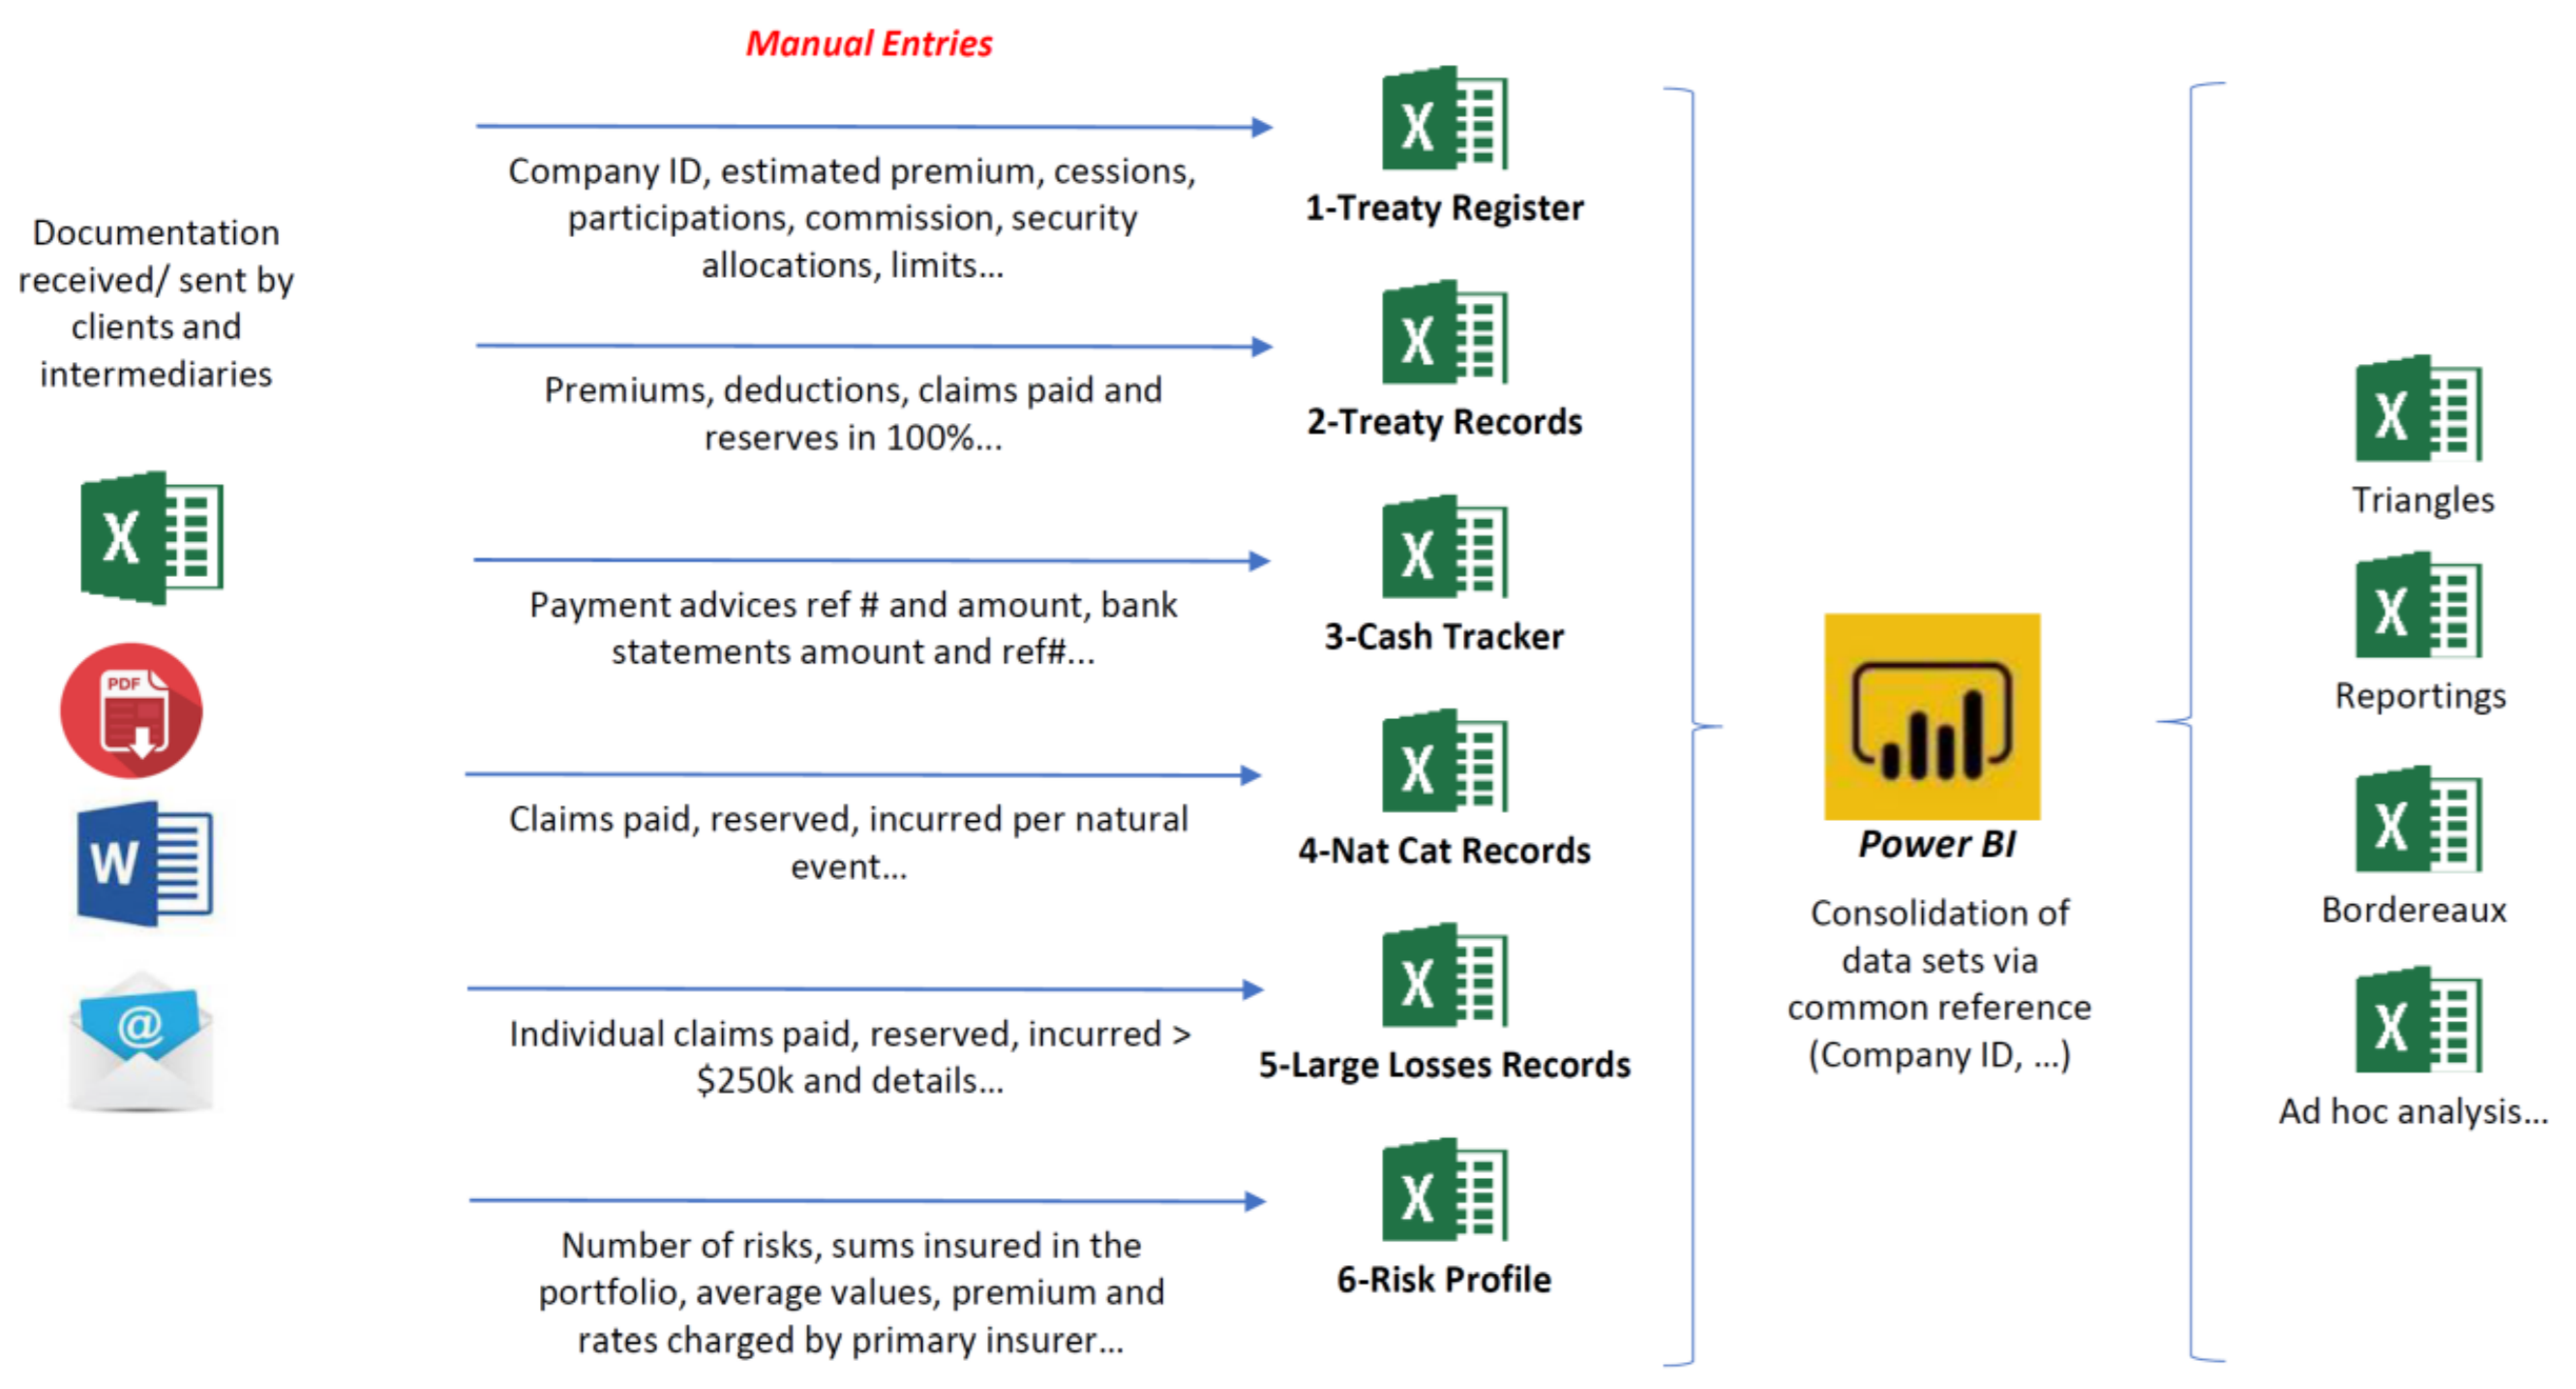
\includegraphics[width=\linewidth]{current_workflow.png}
    \caption{The current workflow at AM RE.}
    \label{fig:current_workflow}
\end{figure}

\begin{enumerate}
    \item Treaty Register: records of individual quota share contracts terms and conditions (estimated income to be generated by the contract, commissions, cessions, individual reinsurer’s securities participation...). Information is entered in 100\% and for AM RE’s participation.
    \item Treaty Records: records of individual quota share contracts results (premiums, claims, commissions, reserves...) on a monthly or quarterly basis. Information is entered in 100\% and for AM RE’s participation.
    \item Cash Tracker: records of balances (Premiums Received –Claims Paid) due by/ owed to the clients. Reconciliation of balances with statements of remittance issued by brokers and payments in the bank. Calculation of AM RE’s fees.
    \item Nat Cat Records: records of client’s total losses incurred, paid and reserved arising from natural perils (storm, fire...). Information is entered in 100\% and for AM RE’s participation.
    \item Large Losses Records: records of client’s individual loss incurred, paid and reserved $>$ \$250,000 for AM RE’s participation. Information is entered in 100\% and for AM RE’s participation.
    \item Risk Profile: records of individual quota share contract underlying portfolio (\# risks, sums insured, average sums insured, premiums). Information is entered in 100\% and for AM RE’s participation.
\end{enumerate}

\subsection{Issues with the Current Workflow}
\begin{itemize}
    \item Storing all the data in Excel implies a lot of manual entries which are a source of human errors.
    \item Contextual information must be entered manually each time an entry is made in a dataset to create relationships between datasets under Power BI or Pivot Tables (eg.Client ID, Underwriting Years, line of business, reporting periods...).
    \item Entries must be entered in 100\% and for AM RE’s participation creating more room for errors.
    \item Data entry process is tedious and time consuming.

    \item Due to the nature of Excel, there is no audit trail of modifications of entries, whether the modification is made accidentally or intentionally.
    \item Excel does not allow for several users to access and make entries to the same dataset at the same time, which creates bottlenecks in the data entry process (especially record keeping of results).
    \item AM RE receives about 50 attachments or emails containing information relevant for the business daily (account statements, bordereaux of premiums and claims, advice of payments or other...). These documents are filed manually and are not “linked” to the entries in the data sets as it could be in a system.
    \item Due to the diverse currencies manipulated, fee calculations rules (one for each security) and status of entries this system has become too complex and is no longer viable.
\end{itemize}



\section{Summary of Literature Review}

Upon further research, these growing pains are common to many companies during their lifetimes. Common solutions were analysed and summarised in the following section.

\subsection{Existing Solutions}

Looking into off-the-shelf solutions was unfruitful as the majority of existing software is aimed at primary insurance rather than reinsurance businesses. The few other companies which operate in a similar fashion to AM RE have hired their own in-house development teams to build bespoke solutions for their specific workflows.

The only other option is to use general business Software as a Service (SaaS) Solutions.
% TODO either include existing solutions from lit review or summarise

\section{Project Specification}
After discussing the problem and research of existing solutions with the client, it was agreed that the best solution would be to build a full bespoke web-based data/administration system. In order for the solution to be successful, it will need to satisfy the following requirements:

\subsection{Requirements}

\subsubsection*{Data Entry}
Users must be able to add, edit and delete:
\begin{itemize}
    \item Securities (Reinsurers)
    \item Binders (Binding Authority contracts)
    \item Treaties (Reinsurance contracts)
    \item Statements (Monthly/quarterly reports for each treaty)
\end{itemize}

\subsubsection*{Multi-user Access}
Allow multiple users to visualize and enter/edit separate data entities simultaneously.
\subsection*{Access-control/security}
Only certain users must be able to view/edit specific parts of the data using login credentials.
\subsection*{Audit History}
The system must automatically record a history of any changes made to data so that there is accountability for changes made.
\subsection*{Backups}
Automatically take snapshots of all the data so it can be restored/viewed at any point in time.
\subsubsection*{File Organisation}
Be able to upload related files/attachments into the system so that they can be quickly viewed rather than having to find the files in a separate file system.
\subsubsection*{Relational Data Consistency}
Automatically handle relations between data to prevent human errors.
\subsubsection*{Real-Time Data Aggregations}
Automatically update aggregations on the data whenever changes are made in real-time.
\subsubsection*{Import Excel Data}
Import the existing spreadsheet data automatically so that it can be re-imported at any time during the test period.

\subsection{Specification changes}
Since the specification was first defined, there have been some modifications.

\subsubsection*{Nat Cat \& Large Loss Data Entry}
It was deemed unnecessary by the client to incorporate this into the system as it was going to be phased out of AM RE's workflow.
\subsubsection*{Automatic Borderaux Generation}
Borderaux are reports which are sent to the securities every quarter. Originally, we had decided that this could be incorporated into the system, however, upon further investigation we realised that this would not be feasible as each security requires a different format of report.
\subsubsection*{Payment Tracking}
Originally, we had planned to incorporate the tracking of payments (handled by the Cash Tracker spreadsheet) into the proposed system. However, the Accounting department later decided that they needed the flexibility that spreadsheets provide in order to continue operating. This was further discussed during a meeting with the CFO who also agreed that this should be handled outside of the system.

\section{Design \& Implementation}
\subsection{Database}
The most complex part of this project is to analyse how the business data links together and how it will be stored in our application. It was decided in the literature review that using the MeteorJS framework would be the best fit for this application. According to the Meteor documentation \cite{meteor_collections_guide}, Meteor only supports MongoDB as a database so this would be used as our storage medium.

A large amount of time was spent with the client going through the existing data structures stored in the Excel spreadsheets and deciding what was necessary to keep and how the data would be stored. After numerous iterations, we came up with the database structure in Figure \ref{fig:database}.

\begin{figure}
    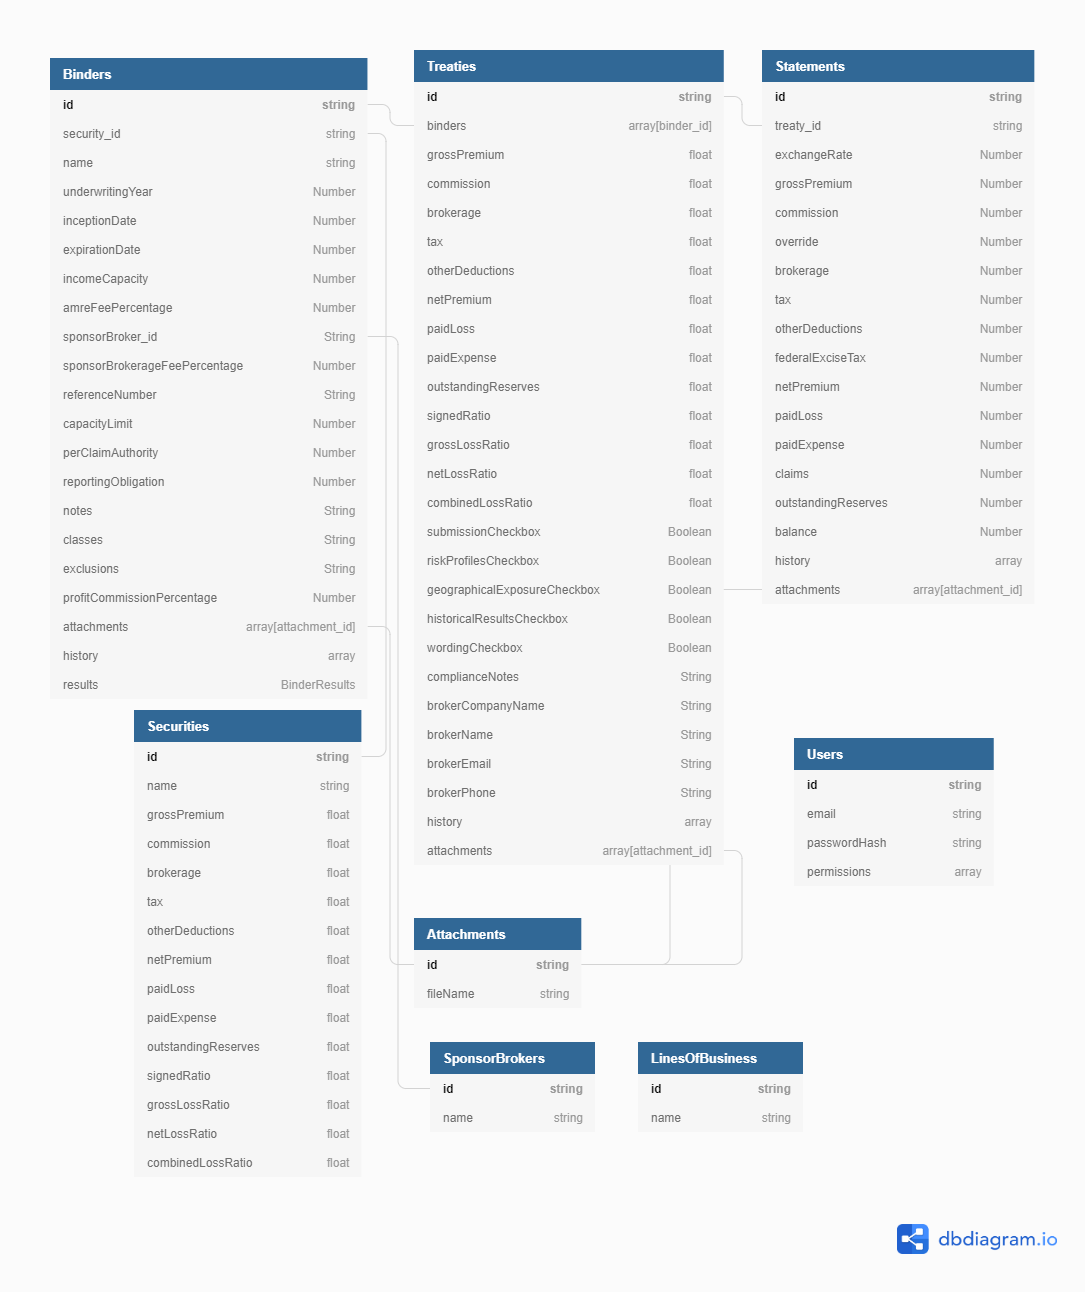
\includegraphics[width=\linewidth]{database.png}
    \caption{Database structure diagram.}
    \label{fig:database}
\end{figure}

It is important to note that MongoDB automatically create the id's which are required. Also, some fields for example history is of flexible type which allows us to store any structure data within. This is necessary as it is impossible to predetermine the format of the changes.

The next step was to import all the existing spreadsheet data into the database. A script was written making use of a spreadsheet parsing library, SheetJS \cite{sheetjs}, to insert and check the data into the database.

This task ended up taking much longer than expected as the data verification checks ended up surfacing a huge number of inconsistencies in the existing data. These had to be rectified by hand which was very time consuming for the Analytics Team however it served as a perfect example of why a better system needed to be developed.

While the aggregate results in the securities, binders and treaties can all be calculated dynamically, we decided to denormalise the results as a caching mechanism. This is because calculating the aggregations is very computationally intensive and it does not make sense to do these calculations every time a client requests the data as the results may not have actually changed if the underlying data is the same.

\subsection{API}
The API is used to perform all the application business logic and provides a layer on top of the database. This allows us to perform authorisation checks as well as data validation which is vital for security, rather than directly allowing clients to write to the database.

A Meteor package called Astronomy\cite{astronomy} was used to provide the API layer. Astronomy was chosen as it is tightly integrated with Meteor and has built in support for validation. It can also be run on both server and client side which allows us to perform client side validation first using the same validation codebase. Once the client side validation has succeeded, the same checks are performed on the server side before any data is actually written to the database for security reasons.

A major feature of Astronomy is it's ability to find the difference between two documents. This is key as it allowed us to easily calculate the difference between the same document before and after a change has been made. These differences can then be written to the document history array, providing the audit trail feature requested by the client.

All the aggregation calculations are also performed in the API layer. Astronomy has an events system which allows us to run code before or after a document is saved. We made use of this when triggering efficient recalculations. For example, if a single statement is modified or added, only the linked treaty needs to be recalculated. When a treaty is modified or recalculated, only the relevant binders need to be recalculated. When a binder is modified or recalculated, only the relevant Security results need to be recalculated. By hooking into Astronomy's afterSave event, we were able to efficiently trigger recalculations on only the relevant documents, greatly reducing the computational cost of database writes.

Additionally, statement level results are always stored in local currency. However this is an issue when calculating treaty level results because a treaty can have many statements all of differing currencies. Therefore all statements need to cache their results in USD as well as local currency. This calculation was easily done as a beforeSave event hook on each statement.

\subsection{User Interface}
It was specifically requested by the client that the user interface had to be modern, clean and responsive. Therefore the decision was made to use ReactJS \cite{react} as the front end library because of it's huge popularity and excellent documentation. React's philosophy is based around creating re-usable components which allowed us to easily break down complex UI features into smaller blocks which can be tested independently.

As the UI library, MaterialUI \cite{material_ui} was chosen because of it's modular component-based structure as well as it's clean, modern design.

\subsubsection{Login Page}
The purpose of the login page is to allow users to authenticate themselves. It acts as security layer and clients are automatically redirected to this page when they are not logged in. The page has an email field, password field and a button to sign in. It's design can be seen in Figure \ref{fig:login}. The page also displays error messages should the user's credentials be incorrect.

\subsection{Securities Page}
% TODO: expand on page layouts

\subsection{Project Structure}
In order to maintain an organised structure, the source code was split into the following hierarchy:
\begin{itemize}
    \item client: the client side starting point
    \item server: the server side starting point + any server side only code that we want to hide from the client.
    \item tests: unit and end-to-end tests
    \item imports \begin{itemize}
              \item api: application business logic
              \item ui: user interface components
          \end{itemize}
\end{itemize}

\subsection{Deployment}
In order to run the application in production, we made use of a number of different platforms. For the database, we opted for a hosted database-as-a-service platform, MongoDB Atlas \cite{mongodb_atlas}. This was chosen because it provides a three node replica set with continuous snapshots every 12 hours. As the database is the most valuable asset, it is necessary to have these snapshots as a failsafe as well as the increased security of a managed service.

\section{Testing}
\begin{itemize}
    \item Technologies used
    \item Unit Testing
    \item E2E Testing
    \item Load testing
    \item Coverage
    \item CI/CD
\end{itemize}

\section{Development Process}
\begin{itemize}
    \item Methodology (kanban) + gantt chart
    \item Version Control
\end{itemize}

\section{Evaluation}

\section{Summary}

\section{Appendix}

\begin{figure}
    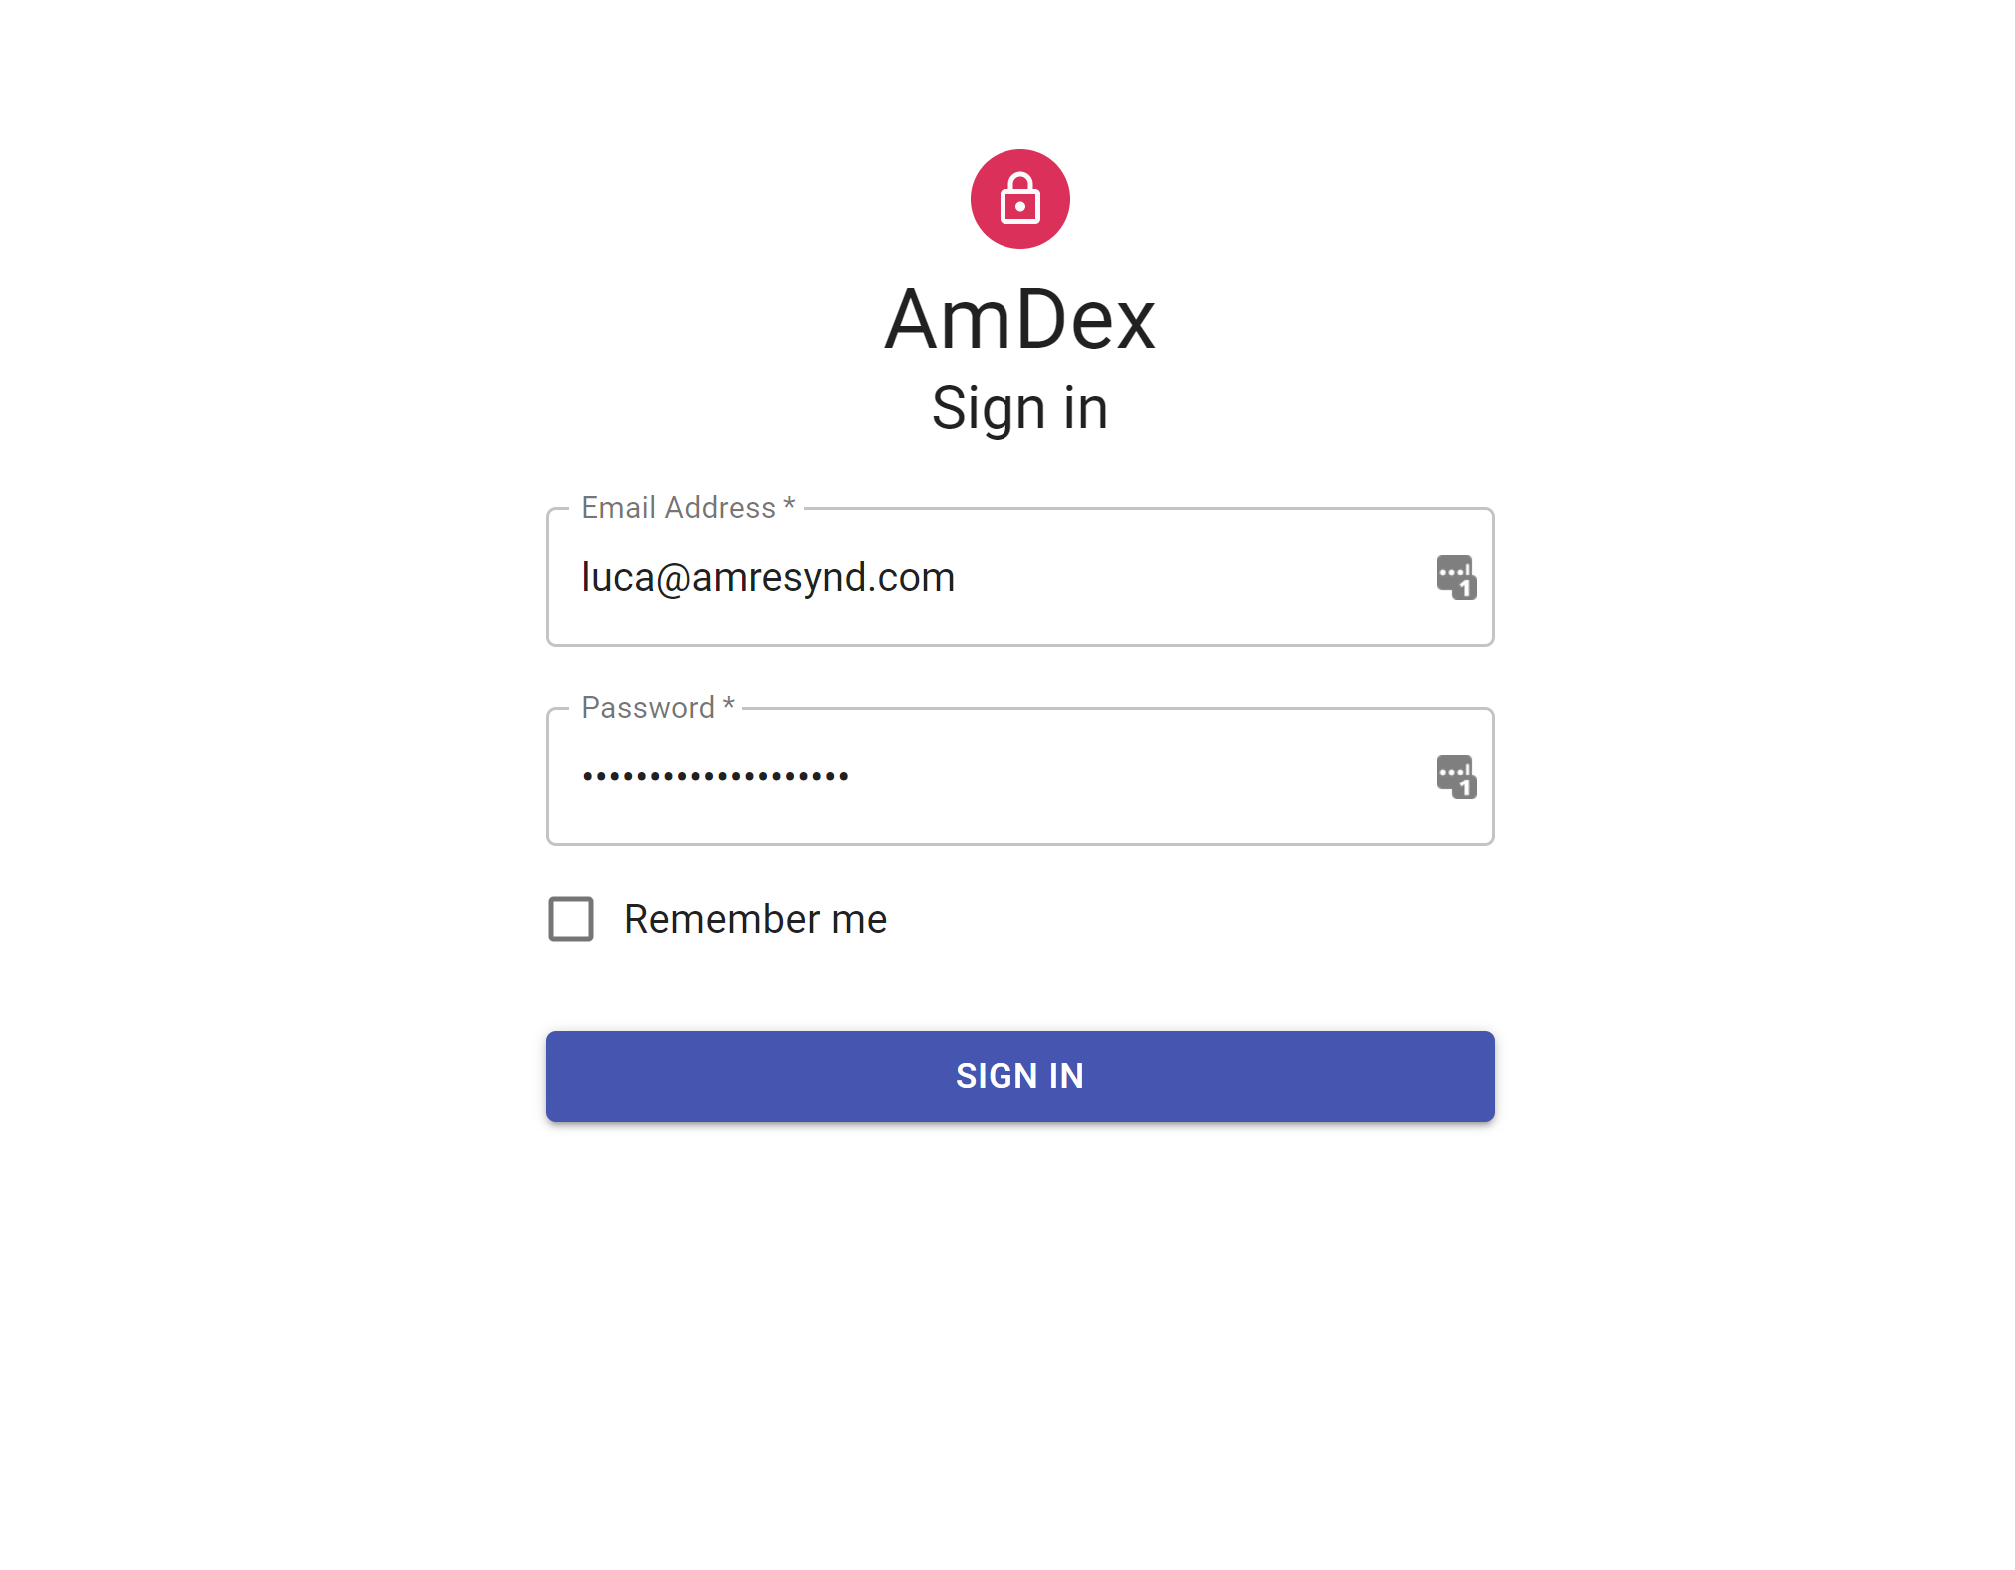
\includegraphics[width=\linewidth]{login.png}
    \caption{Login page design.}
    \label{fig:login}
\end{figure}

\begin{figure}
    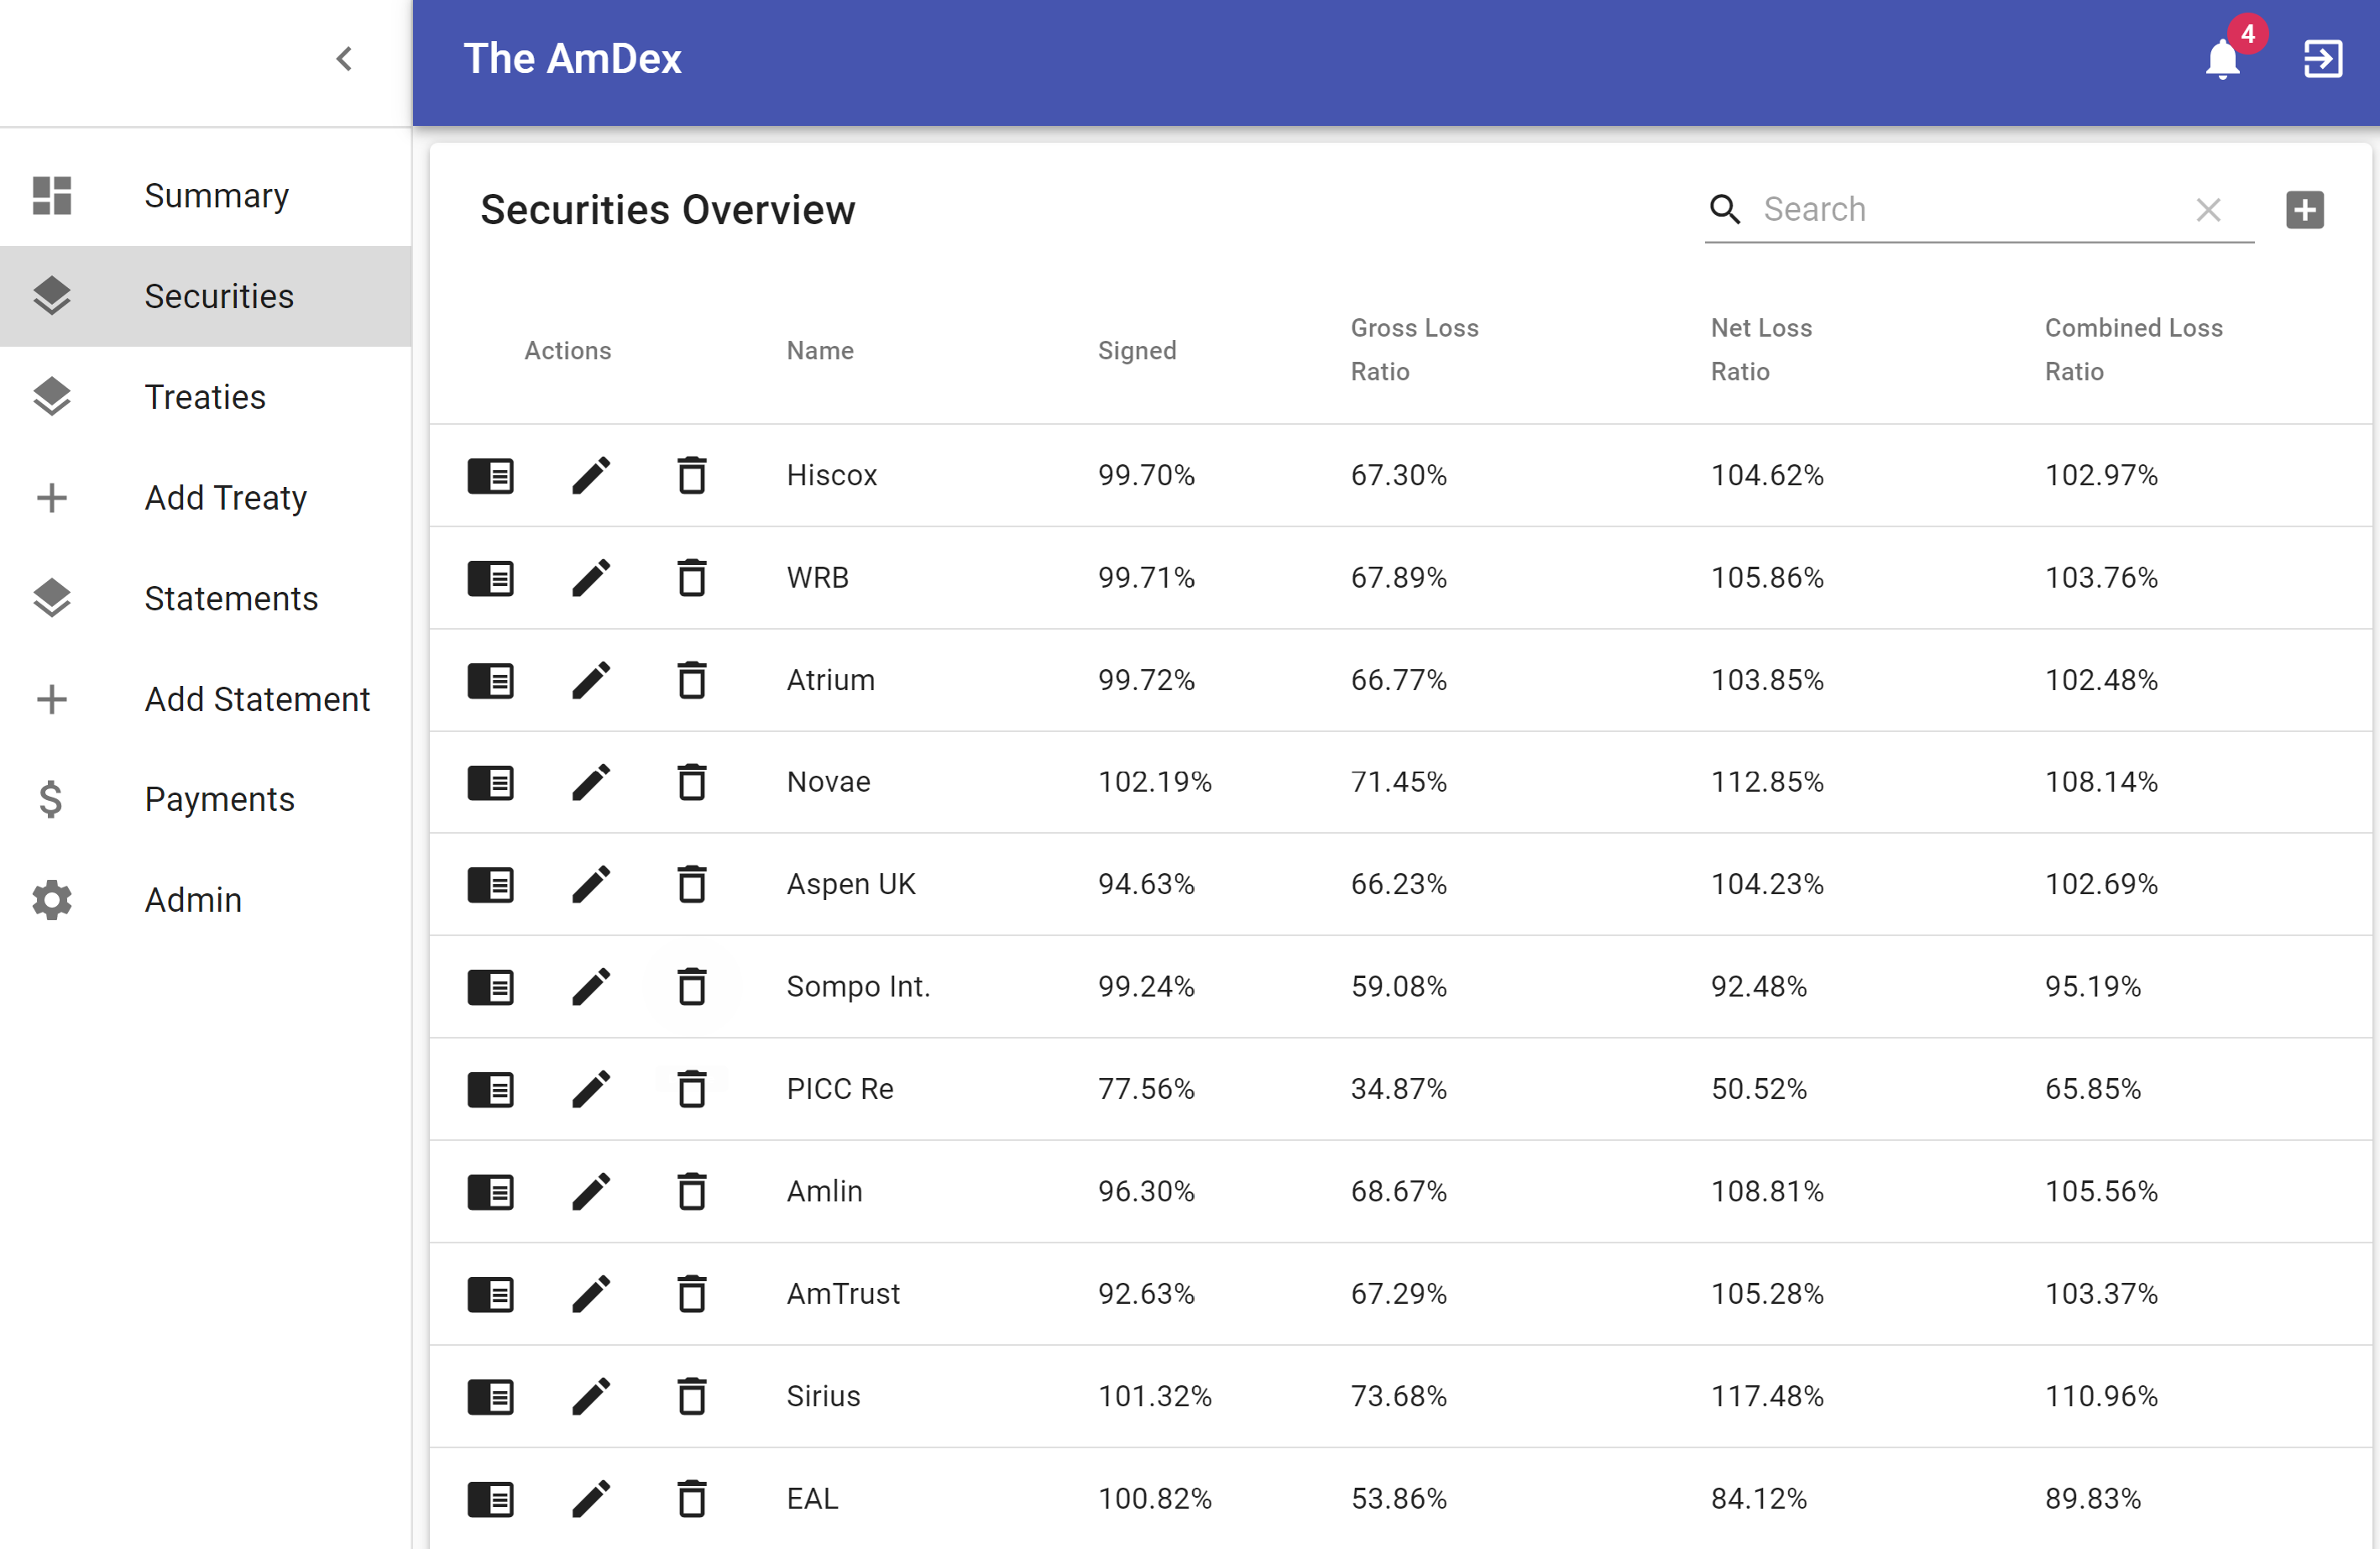
\includegraphics[width=\linewidth]{securities.png}
    \caption{Securities page design.}
    \label{fig:securities}
\end{figure}

\bibliography{dissertation}
\bibliographystyle{IEEEtran}

\end{document}
